\documentclass{pnastwo}
\usepackage{pnastwoF}
\usepackage[numbers,round]{natbib}
\usepackage{graphicx}
\usepackage{amssymb,amsfonts,amsmath}
\usepackage[american]{babel}
\usepackage{color}

\newcommand{\red}[1]{\textcolor{red}{#1}}

\include{preamble}

% \authornote{Please address correspondence to: 

% \vspace{12 pt}
% Daniel Yurovsky

% Jordan Hall (Building 420)

% Stanford University

% 450 Serra Mall

% Stanford, CA 94305

% \vspace{12 pt}
% Email: yurovsky@stanford.edu 

% \vspace{12 pt}
% Word Count: 1999

% References: 40}

\begin{document}

\widowpenalty10000
\clubpenalty10000

\title{Developmental Changes in the Speed of Social Attention in Early Word Learning}
\author{Daniel Yurovsky\affil{1}{Department of Psychology, Stanford University}, Anna Wade\affil{2}{School of Medicine, University of California, San Francisco}, Allison M Kraus\affil{1}{}, Grace W. Gengoux\affil{3}{School of Medicine, Stanford University}, Antonio Hardan\affil{3}{}, \and Michael C. Frank\affil{1}{} }
\contributor{Submitted to Proceedings of the National Academy of Sciences
of the United States of America}

% \affiliation{Department of Psychology, Stanford University}
% \shorttitle{Synthesizing Cross-Situational Learning}
% \leftheader{Yurovsky \& Frank}

% \abstract{}

\maketitle

\begin{article}
\begin{abstract}
To begin learning the meaning of a word, a child must determine if this word is being used to refer to something in the immediate physical context. Social cues---like the eye-gaze of a helpful speaker---are powerful information sources for resolving this problem. Studies of children's gaze following have generally been concerned with its developmental origins, demonstrating measurable success in early infancy. We show that this ability has a long developmental trajectory, however: Slow, continuous improvements in speed of social information processing occur over the course of the first 5 years of life. This developing ability is a significant bottleneck on early word learning, predicting changes in children's learning of new words over the same time period. Finally, we show that the same bottleneck exists in children diagnosed with autism spectrum disorders. These results describe a route by which increases in social expertise can lead to changes in language learning ability and highlight the dependence of developmental outcomes on not just the existence of particular competencies but their proficient use in complex contexts.
\end{abstract}
\keywords{ language acquisition | word learning | social cues}

\subsection{Significance Statement}
The study of language development has historically focused on pinpointing children's earliest points of competence in each domain. Learning outside the laboratory is ultimately controlled by proficient use of these same mechanisms, however. While infants can follow social cues like eye-gaze early in their first year, we show that the speed and fidelity of this process improves continuously over the first five years of life. The problem of tracking social information is far from resolved for young infants; it remains a bottleneck on word learning for typically developing children into the preschool years and and does so for autistic children as well. This work highlights the importance of studying not just origins but also the developmental trajectories of higher-level cognitive processes.

\vspace{12 pt}

\dropcap{C}hildren's first five years are a time of rapid developmental change. One striking development is children's growing mastery of their native language. The typical child will go from saying her first word shortly before her first birthday to producing complex, grammatical sentences only a few years later. Perhaps because of the fundamentally discrete nature of the units of language itself, much work in language acquisition has focused specifically on the origins of these important abilities \cite[but c.f.][]{fernald1998,port2005}. Reviews of language development are generally a list of milestones: e.g., infants acquire the ability to use sequential statistics to segment speech at 8 months \cite{saffran1996}, begin to use co-occurrence statistics to learn word-object mappings at 12 months \cite{smith2008}, and begin to use syntax to infer the meanings around 24 months \cite{gertner2006}. New exciting work then is often a demonstration of some competence earlier than previously observed \cite{bergelson2012}. This research strategy stands in contrast to work in domains like visual and motor development, in which researchers have sought to measure continuous changes in children's abilities as they develop \cite{sokol1978,banks1980,forssberg1991,thelen1995}.

Here we take as a case study children's use of social information to infer the meanings of new words. Over the first five years, children acquire a productive vocabulary of approximately 4000--5000 words \cite{goulden1990}. Though these words belong to many grammatical categories, a large proportion are concrete nouns \cite{bates1994}. While acquiring a fully adult-like meaning for any of these nouns likely unfolds over multiple encounters, the very first problem a child faces when hearing a new word is referential uncertainty: Does the word refer to something in the current situation, and if so, what \cite{carey1978, yu2007, frank2009}? A powerful source of information for resolving this uncertainty is available in the social cues provided by the speaker: e.g., where is the speaker looking? Consequently, a large body of research has accumulated documenting young infants' abilities to track a speaker's social cues and use them to infer the target of her reference \cite[e.g.][]{scaife1975, baldwin1993, hollich2000, senju2008}.

This research has focused almost exclusively on discovering the earliest point of infants' competence in using social information. Underlying this focus is an implicit assumption that, once the general ability to use social cues is demonstrated, children's proficiency with processing these cues is relatively high \cite[e.g.][]{corkum1998, brooks2005, csibra2009}. Contradicting this assumption, however, some work has argued that rapid gaze-following may occur relatively rarely in natural interactions and may be difficult even for older children and adults under some circumstances \cite{loomis2008, vida2012,yu2013}. 
% Because higher-level cognitive processes like social inference and word learning must sit on top of lower-level cognitive architectures that change continuously over development, they must themselves show significant change beyond their early origins.

There are more basic reasons to assume that children's use of social information in word learning would have a protracted developmental trajectory, as well. Using social information to resolve referential uncertainty is a highly time-sensitive process of continuous re-allocation of attention between the speaker and the objects in the context. To learn from a given situation, learners must rapidly process the auditory and visual information they are receiving. Consequently, competence is not enough: the referential uncertainty problem should remain a problem in proportion to a child's developing ability to control her attention, process auditory and visual information, and hold the information in memory \cite{dempster1981, kail1991, gathercole2004}. 

\begin{figure}
        \includegraphics[width=.45\textwidth]{figures/heatfigure.pdf}
        \includegraphics[width=.5\textwidth]{figures/reflook_learning.pdf}
	\caption{\label{fig:reflook_learning}  (top) Example frames from the first word learning dialogue in Experiment 1. Each image shows the regions of interest used for later analysis (white boxes) and a heat map of the entire participant group's average point of gaze (hotter colors indicate more fixation; scale is constant across frames). \red{rename heatmaps} (bottom) Looking to target vs. competitor objects during the learning portion of Experiments 1 (typically-developing children) and 2 (ASD children), plotted by phase of the naming event. Points show means and error bars show 95\% confidence interval across participants; points are offset on the horizontal to avoid overplotting.}
\end{figure}

In three experiments, we test the hypothesis that social attention allocation is a bottleneck in early word learning. We constructed videos that used novel words in a series of naturalistic object-focused dialogues and monologues. These videos were intended to be sufficiently difficult in their structure that in-the-moment disambiguation would pose a significant challenge to young learners, yet sufficiently simple that co-occurrence information could allow for successful word learning. We measured children's eye-movements during viewing as an index of their online inferences about the current conversational referent, and then tested their retention of the words they learned via a series of forced-choice test trials. These rich time-course data allowed us to test the hypothesis that those children who were successful in attending to the conversational referent would be the same children who learned and retained the words. 

In Experiment 1, we measure developmental changes in social information processing and use these to predict word learning in typically developing children. In Experiment 2, we tested a sample of children diagnosed with autism spectrum disorder in the same paradigm as Experiment 1 to determine if social attention was a bottleneck on their learning from these videos in the same way as for the typically developing children. In Experiment 3, we manipulate the timing of social information directly to test the causal role of fast social attention, again in typically developing children. In all three studies, we recruit children across a broad age range, giving us the power to see continuous changes in both social attention and novel word learning. 

\section{Experiment 1: Social Attention and Word Learning}

Experiment 1 was designed to estimate the developmental trajectory of children's online social information process in complex interactions, and to ask whether this processing had downstream consequences for word learning. The experiment consisted of two parts: learning and test. During the learning part, participants watched a series of dialogues and monologues by an actor and an actress in which they introduced and discussed two novel objects and two familiar objects. Each video contained two naming sequences (pictured in Fig.~\ref{fig:design}, top); these sequences were broken into a series of phases during which the speaker named, looked at, named again, and reached for a particular object, allowing for the separate measurement of name-, gaze-, and reaching-related changes of attention. 

We first measured the proportion of time participants spent looking at the target referent during the naming sequences in which the novel objects were introduced (Fig. ~\ref{fig:design}). Children in all age groups, as well as adults, showed an increase in looking to the correct referent over the course of these naming sequences, with looking reaching nearly 100\% by the end of these events after the speaker had made contact with the toy. To determine whether there reliable were age-related differences earlier in the naming sequences, we fit a mixed-effects models predicting proportion of looking to the target referent from age, phase, and their interaction. This model showed no main effect of age, but a significant interaction between age and the gaze-following phase (after the speaker turned to look at the intended referent; $\beta_{interaction} = .065$, $t = 3.54$, $p <.001$; for full regression table see \emph{SI: Regression Analyses}). While the youngest children were only occasionally able to follow gaze during this short interval, older children and adults showed much stronger changes in gaze behavior. Thus, the ability to follow a speaker's gaze online in a naturalistic conversation appears to develop significantly over the course of the first five years, and even further into adulthood.

Next, to measure children's retention of the novel words they were exposed to during the learning portion of the experiment, during the test trials we showed them pairs of toys and labeled one, using a standard looking-while-listening procedure \cite{fernald1998,fernald2008}. To measure online language comprehension more generally, we also included familiar word trials. Although familiar trials were easier than novel trials for children in all age groups ($\beta_{novel} = -.13$, $t = -9.25$, $p <.001$;), preferential looking to the target referent increased on both familiar and novel trials ($\beta_{age} = .065$, $t = -9.44$, $p <.001$). See \emph{SI: Timecourse Information} for time-course information across age groups. 

Was older children's improved performance in retaining word-object mappings a result of improvements in social information processing abilities? To test this hypothesis, we constructed a mixed-effects regression model, predicting children's preferential looking on bovel trials from their proportion of looking to the target referent during naming events. Referential looking to the target during the window after the speaker fixated the novel referent was a highly reliable predictor of word learning (\red{stats}). Furthermore, this predictor mediated the effect of age in the model: Knowing the proportion of time a child spent looking at the referent in this look window captured all of the variance previously accounted for by age. Thus, age-related improvements in social attention, whatever their cause, are a critical bottleneck on learning from naming events throughout early childhood. Put another way, the age-related changes in word learning that we saw appeared to be accounted for largely by changes in social attention.

\section{Experiment 2: Social Attention in Autistic Children}

The naming events in Experiment 1 contained information sufficient to infer the meanings of the novel words at two timescales: (1) within the interactions, by following the informative social cues, and (2) across the interactions, by using co-occurrence statistics between the words and objects. While typically developing children's social information processing predicting a large chunk of the variance in their word learning, it is possible that atypically developing children would use a different strategy.

We tested an additional group of 50 children diagnosed with Autism Spectrum Disorder who, due to deficits in social information processing, might be expected to learn predominantly from the cross-situational statistics instead. These children did indeed process social information less efficiently---following the speaker's gaze no better than the youngest children in our sample (Fig.~\ref{fig:reflook_learning}. They also learned learned the Novel words, and attended to the referents of Familiar words at approximately the same levels (Fig.~\ref{fig:reflook_test}). While age was uncorrelated with word learning for the Autistic children ($r = 0$), following the speaker's gaze was highly predictive of Novel word learning ($r = .51$), just as in the typically developing sample. Thus, social information processing remains a critical bottleneck on word learning in autistic children, just as in typically developing children.


\begin{figure}[b]
	\center{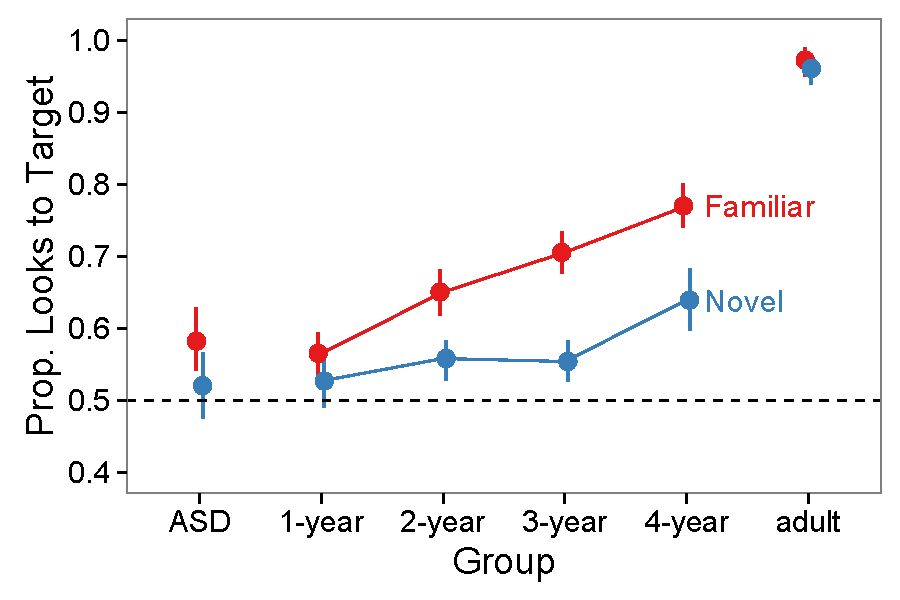
\includegraphics[width=.5\textwidth]{figures/reflook_test.pdf}}
	\caption{\label{fig:reflook_test} Test trial performance in Experiment 1, plotted by participant group. Colors show familiar and novel word trials. Error bars show 95\% confidence intervals across participants. Points are offset on the horizontal to avoid overplotting.}
\end{figure}

\section{Experiment 2}

The naming events in Experiment 1 provided children with a number of informative cues to the referents of the novel words: social gaze, speaker's manual interaction, and also cross-situational co-occurrence statistics. Our analysis showed that fast processing of social gaze was the primary predictor of ultimate word learning. In Experiment 2, we tested this prediction directly. 

In Experiment 2, the two Novel words were introduced in two different kinds of naming events. In Extended Hold events, the speaker made contact with and manipulated the target toy for the duration of the naming event, providing an extended cue to the target of her referential intention. In contrast, on Brief Look trials, the speaker only provided punctate gaze information, looking to the target of her referential utterance briefly after naming it and then looking forward towards the camera for the remainder of the naming event. On the basis of the results from Experiment 1, we predicted that Extended Hold trials would show less developmental differentiation in social attention and be easier to learn from. In contrast, we predicted that the Brief Look trials would be more difficult, and that gaze-following would again mediate age in predicting word learning at test.

As predicted, children's proportion of looking to the target relative to the competitor was consistently near ceiling on Extended Hold trials, and did not differ across development just as in the Contact-End window in Experiment 1. In contrast, children were less successful at locating the target of the speaker's social cue on Brief Look trials, and their ability to do so improved markedly across development  just as in the Name-Look window from Experiment 1. 

As before children's preferential looking to the target on test trials was higher for Familiar words, and improved across development for both Familiar and Novel words. In addition, as predicted, performance on test trials for the word introduced in Extended Hold trials was better than for the word introduced in Brief Look trials, indicating that children learned more when they did not have to rapidly process the speaker's social cue, but could use it for disambiguation over the course of the whole naming event.

As in Experiment 1, we constructed a mixed effects model predicting children's test performance from their age and referential looking during naming events. As predicted, we found that referential looking was a significant predictor of learning, and mediated age on Brief Look trials. In contrast, referential looking was not a significant predictor, although age was on Extended Hold trials. Together, these results confirm the social information processing bottleneck hypothesis. Although many processes are involved in learning the meaning of a novel word---processing the fluent speech in which it is embedded, encoding the referent it labels, and retrieving and remembering it across multiple encounters---a critical first bottleneck is locating the intended referent in the moment of the word's use. 

\begin{figure}[h]
	\center{\includegraphics[width=.5\textwidth]{figures/socword_test.pdf}}
	\caption{\label{fig:reflook_test} Test trial performance in Experiment 2 for the Brief Look and Extended Hold conditions; familiar trial performance is averaged across both conditions. Error bars show 95\% confidence intervals; \red{points are offset on the horizontal to avoid overplotting.}}
\end{figure}

\section{Discussion}

\begin{materials}

\subsection{Participants} Data from typically-developing children was collected at the San Jose Children's Discovery Museum, where parents and their children were invited to participate in an experiment investigating children's early word learning. In Experiment 1, we collected both demographic and eye-tracking data from 343 children in the target age range (1 -- 5 years), of whom 113 were excluded from the final sample for at least one of the following reasons: developmental issues (N=7), experimental issues including sibling interference (N=17), reported household English usage less than 75\% (N=44), or unacceptable calibration (N=58). Our final sample included 229 children, ages 1 -- 5 (M=3.2 years; age 1 -- 2: N=35, age 2--3: N=60, age 3--4: N=72, age 4--5: N=62; 115 girls). In Experiment 2, we collected both demographic and eye-tracking data from 343 children in the target age range (1 -- 5 years), of whom 113 were excluded from the final sample for at least one of the following reasons: developmental issues (N=7), experimental issues including sibling interference (N=17), reported household English usage less than 75\% (N=44), or unacceptable calibration (N=58). Our final sample included 229 children, ages 1 -- 5 (M=3.2 years; age 1 -- 2: N=35, age 2--3: N=60, age 3--4: N=72, age 4--5: N=62; 115 girls).

Data from Autistic children was collected at Stanford University, where parents and their children.... we collected both demographic and eye-tracking data from 343 children in the target age range (1 -- 5 years), of whom 113 were excluded from the final sample for at least one of the following reasons: developmental issues (N=7), experimental issues including sibling interference (N=17), reported household English usage less than 75\% (N=44), or unacceptable calibration (N=58). Our final sample included 229 children, ages 1 -- 5 (M=3.2 years; age 1 -- 2: N=35, age 2--3: N=60, age 3--4: N=72, age 4--5: N=62; 115 girls).

Adult participants in Experiment 1 were 17 Stanford undergraduate students who participated in exchange for course credit.

\subsection{Stimulus and Design} Children and adults in both experiments watched a $\sim$6 minute video. For both experiments, these videos began with a short calibration calibration, learning, and test. Calibration began with a short video of a puppet to capture children's attention, and then showed an image of the puppet moving around to two calibration points. Each video also contained learning trials: videos in which speakers seated at a table with two toys provided social cues and labelled one of the toys. Each video also contained test trials in which pictures of two objects were shown on a black background and a voice asked the participant to look at one of them \cite[as in][]{fernald1998}.

In Experiment 1, these learning trials consisted of two dialogues in which two speakers sat at a table together, and one referred to teach of the two novel toys whose names were taught in the experiment (``toma'' and ``fep''). The other two learning trials were monologues in which one of the speakers sat at a table alone, with one of the novel toys and one familiar toy and referred to each in turn. Each naming event consisted of six events: first a naming phrase, the a look at the object accompanied by a comment, a second naming, a reach for the object, and finally a demonstration of the object's function accompanied by a third naming. Each novel object was named nine times in total over the course of the video. Eight tested familiar objects (e.g. dog/car or lamp/carrot); the other eight paired the two novel objects. Naming phrases were of the form ``Look at the [car/fep]! Do you see it?'' and were spoken by the actors in the video.

After these four learning trials, the video contained 16 two-alternative forced-choice trials between pairs of pictures 

In Experiment 2, we simplified the learning trials. All naming sequences were monologues and both toys on the table were novel. Three of the naming sequences these were Extended Hold trials, in which the speaker reached for and interacted with one of the two toys while describing its function and producing its name three times. The other three were Brief Look trials in which the speaker produced the same kind of description but indicated the target toy only with a brief look following the first naming event. Brief Look and Extended hold trials used a distinct but consistent set of two toys, and the same toy was consistently either the target or the competitor on each trial type. In both experiments, the side of the screen on which each toy appeared was counterbalanced across trials.



In Experiment 1, all learning trials occurred before the test trials. 

The test section consisted of 16 two-alternative forced-choice trials between pairs of pictures  \cite{fernald2008}. 
Families were escorted to a small room off the museum floor, where children watched the video from a car seat approximately 60cm from the monitor of an SMI RED 120 Hz corneal reflection eye-tracker (mounted on an adjustable arm). Total experiment duration was approximately 6 minutes. 

\subsection{Data Analysis}

To ensure appropriate precision in region-of-interest analyses, infants' calibrations were corrected and verified via robust regression \cite<described in>{frank2012}, and calibration corrections were assessed by two independent coders ($\kappa = .85$). For maximum accuracy in the analyses reported below, we excluded children whose calibrations could not be verified and corrected.

To assess looking behavior related to interpretation of the conversational referent, we created a measure of  ``referential looking'': how much children looked at an object as it was being described in the word learning clips. We broke descriptions into six time periods (Figure \ref{fig:stim}): a baseline period of exactly 2 s, name 1 to look (M = 1.7 s), look to name 2 (M = 2.0 s), name 2 to initiation of reach (M= 4.8 s), initiation of reach to point of contact (M = .8 s), and after contact with the object (1 s). For each of these, we examined the proportion of total dwell-time that fell in a region-of-interest around the object. 

To measure accuracy on test trials, we computed each child's total dwell time on the target following onset of the labeling word. For maximal comparability across age groups,  we chose a 1500 ms window for the familiar words and a 2000 ms window for the novel words (both beginning 500 ms after word onset). The reliability of individual participants' measurements was related to the amount of data they contributed. We therefore created two exclusion criteria: a strict criterion---in which a participants' measurements for novel or familiar test trials were only included if they had 4/8 trials with $>80\%$ data in each---and a permissive criterion---in which participants were included if they had 2/8 trials with $>50\%$ data). Figures and results in the text use the strict inclusion criterion; qualitatively similar results from the permissive criterion are reported in Supplemental Information.
\end{materials}

\begin{acknowledgments}
We gratefully acknowledge the parents and children who participated in this research and the staff of the San Jose Children's Discovery Museum for their collaboration on this line of research. This work was supported by NIH NRSA F32HD075577 to DY,  and grants from the John Merck Scholars program, the Stanford Child Health Research Initiative to MCF .
\end{acknowledgments}

\bibliographystyle{pnas2011}
\bibliography{refword}

\end{article}

\end{document}
